\begin{figure*}[h] 
\centering 
%	\subfigure[True Pareto Front 9_15 ]
%	{
%		\label{fig:true9_15}
%		\includegraphics[width=0.175\textwidth]{figs/WFG/true9_15.eps}
%	}
%	\hspace{0em}    
	\subfigure[$F$-DEA]
	{
		\label{fig:our9_15}
		\includegraphics[width=0.175\textwidth]{figures/experiments/wfg/our9_15temp.eps}
	}
	\hspace{0em}
	\subfigure[NSGAIII]
	{
		\label{fig:nsgaiii9_15}
		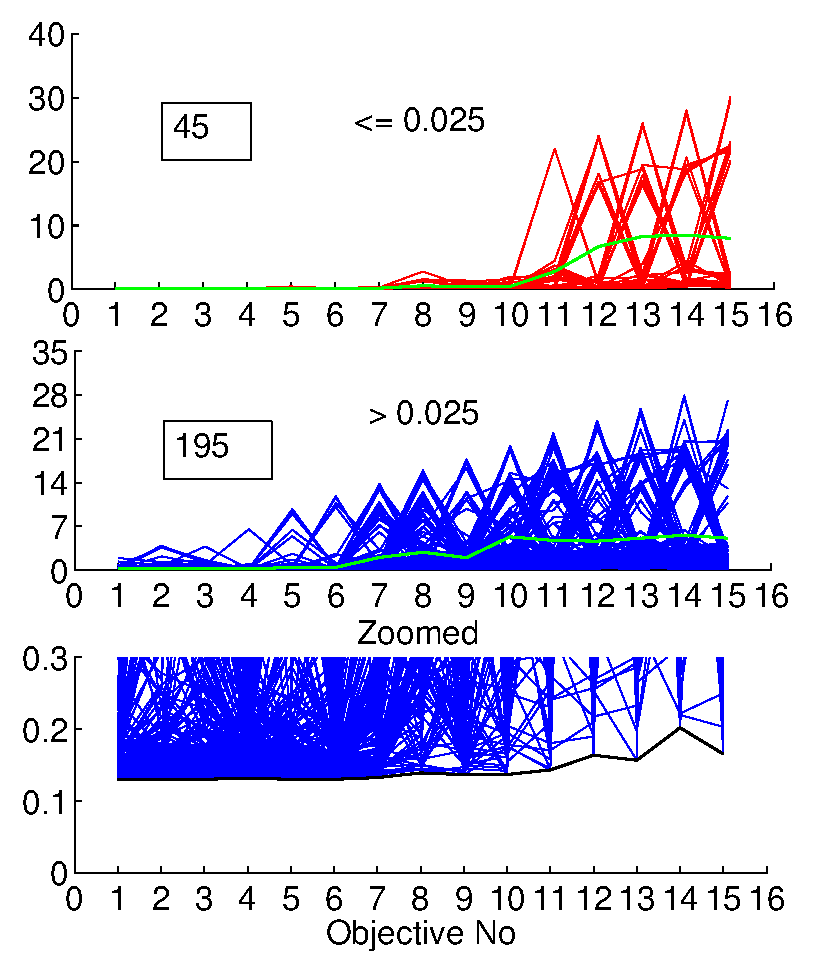
\includegraphics[width=0.175\textwidth]{figures/experiments/wfg/nsgaiiiwfg9_15.eps}
	}	
%	\hspace{0em}
%	\subfigure[MOEA/D]
%	{
%		\label{fig:moead9_15}
%		\includegraphics[width=0.175\textwidth]{figures/experiments/wfg/moeadwfg9_15.eps}
%	}
	\hspace{0em}
	\subfigure[FD-NSGAII]
	{
		\label{fig:zhenan9_15}
		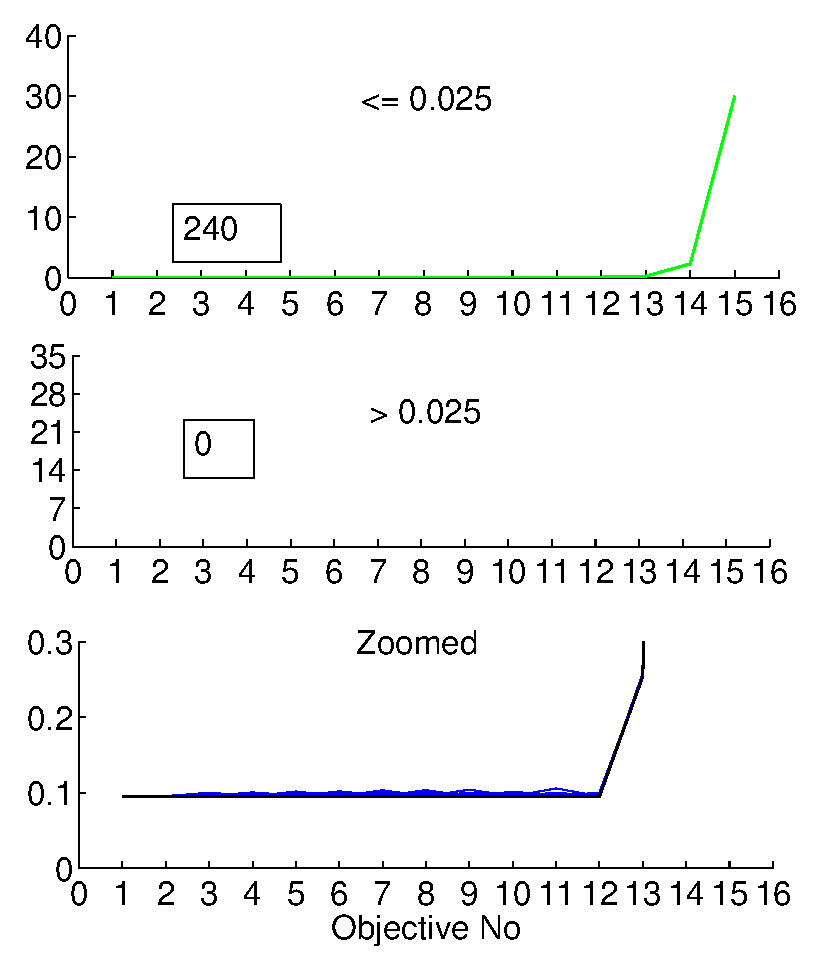
\includegraphics[width=0.175\textwidth]{figures/experiments/wfg/zhenanwfg9_15.eps}
	}
%	\hspace{0em}	
%	\subfigure[HypE]
%	{
%		\label{fig:hype9_15}
%		\includegraphics[width=0.175\textwidth]{figures/experiments/wfg/hypewfg9_15.eps}
%	}
	\hspace{0em}
	\subfigure[SDE]
	{
		\label{fig:sde9_15}
		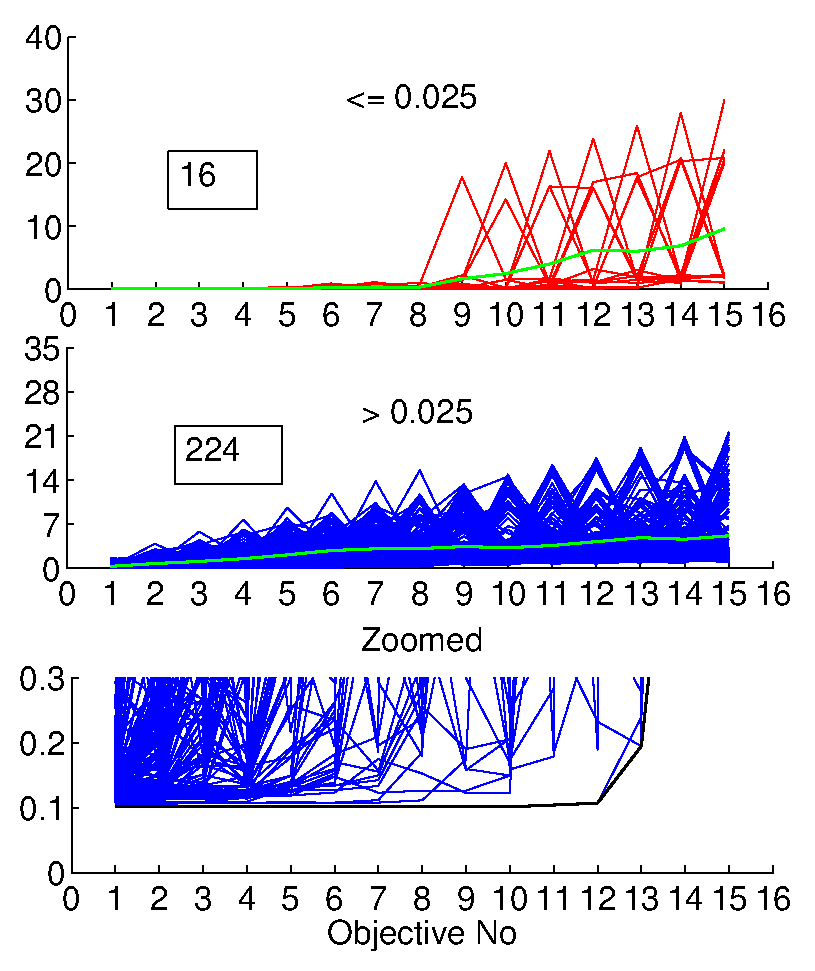
\includegraphics[width=0.175\textwidth]{figures/experiments/wfg/sdewfg9_15.eps}
	}
	\hspace{0em}
	\subfigure[PICEAg]
	{
		\label{fig:piceag9_15}
		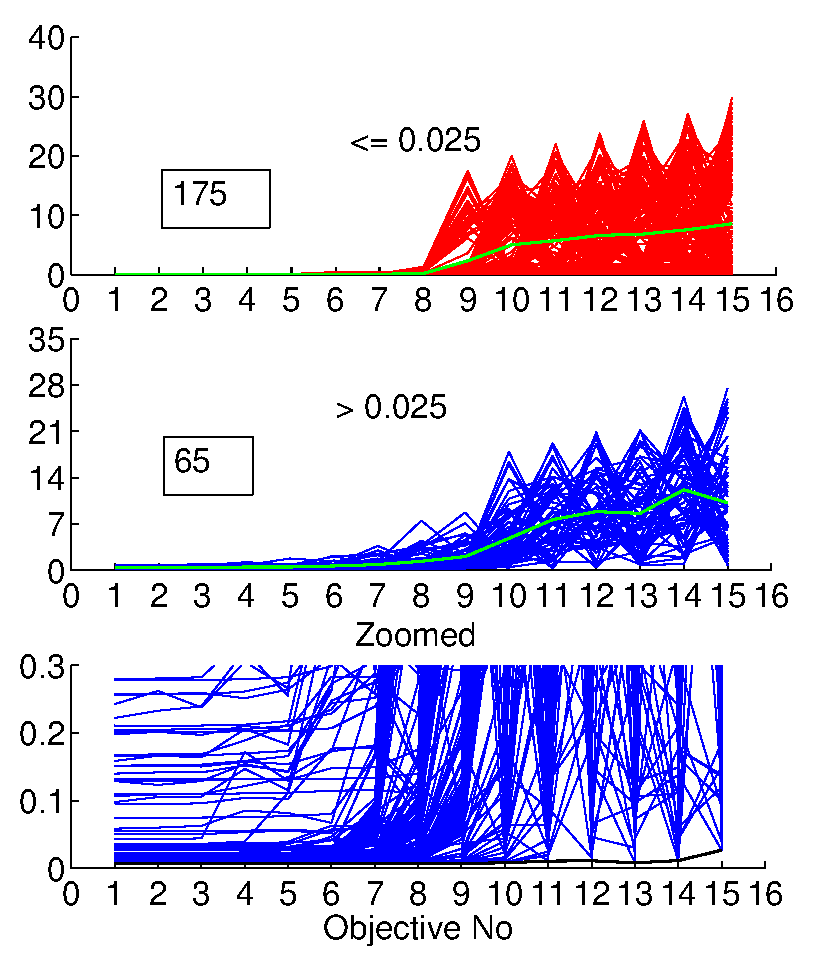
\includegraphics[width=0.175\textwidth]{figures/experiments/wfg/piceagwfg9_15.eps}
	}
	
\caption{Parallel coordinate plot of different algorithms for the WFG9 problem
with 15-objective. Here the non-dominated solutions are separated into two categories based on a threshold distance value from the normalized Pareto front. The solutions with a distance less than or equal to 0.025 is regarded as converged solutions (top figure, red colored), while the other ones are  regarded as non-converged solutions (middle figure, blue colored). Also, to observe the simultaneous minimization of different objectives, the bottom figure shows closer inspection of all the solutions.}
\label{fig:WFG9_15D}
\end{figure*}
